% 数轴上 A=-2, B=5, AB=7
\documentclass[tikz,border=4pt]{standalone}
\usepackage{ctex}
\usepackage{amsmath}
\usetikzlibrary{calc, arrows.meta, decorations.pathreplacing}
\begin{document}
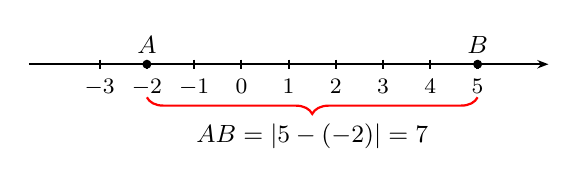
\begin{tikzpicture}[scale=0.6, thick]
  \draw[-{Stealth[length=4pt]}] (-4.5,0) -- (6.5,0);
  \foreach \x in {-3,-2,-1,0,1,2,3,4,5}
    \draw (\x,0.1) -- (\x,-0.1) node[below, font=\footnotesize] {$\x$};
  \filldraw[black] (-2,0) circle (2pt) node[above, font=\small] {$A$};
  \filldraw[black] (5,0) circle (2pt) node[above, font=\small] {$B$};
  \draw[decorate, decoration={brace, amplitude=6pt, mirror}, red, thick]
    (-2,-0.7) -- node[below=6pt, font=\small, black] {$AB=|5-(-2)|=7$} (5,-0.7);
\end{tikzpicture}
\end{document}
